\section{Benchmark audit and evaluation protocol}
\label{sec:method}

We select a suite of \StudyBenchmarkCount{} non-coding benchmarks from 554 candidates and use an AI-assisted audit
pipeline to establish the task, the published reference system, and the conditions of each
comparison (Figure~\ref{fig:audit-pipeline}). The study has two complementary comparisons.
\emph{Direct Codex versus published SOTA} measures performance against the selected system's
paper-reported score; it may combine differences in backbone, scaffold, and evaluation conditions.
\emph{Shared-backbone evaluation} re-runs available specialist systems on our model endpoint to
study the contribution of their scaffolds, with remaining protocol differences declared.
The first comparison supplies Figure~\ref{fig:main-results}; the second requires completed,
audited comparator runs. The comparator evaluations on the 25\% subsets are still running;
unavailable results remain \todo{pending}.

\begin{figure}[t]
\centering
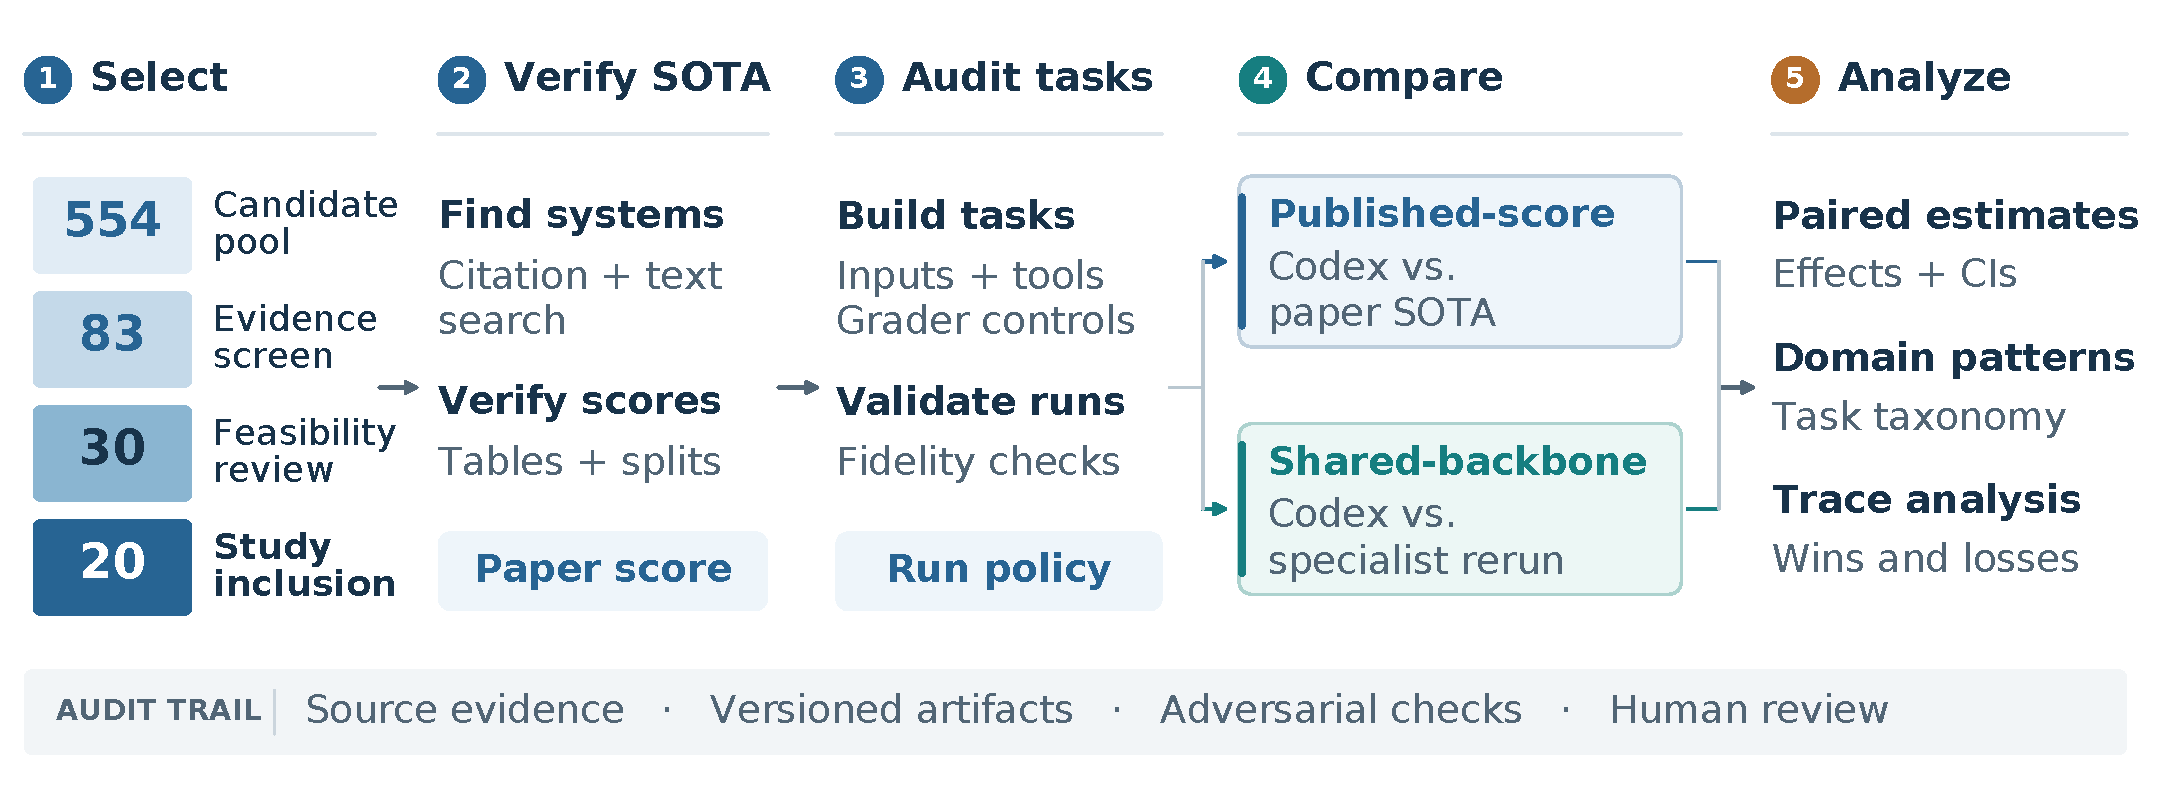
\includegraphics[width=\textwidth]{figures/benchmark_audit_pipeline.pdf}
\caption{The benchmark audit pipeline. Each stage produces reviewable evidence. Published-score
comparisons and shared-backbone re-runs answer different questions; the final stage includes
ongoing comparator evaluations and planned trace analyses. Selection reviews comparator evidence,
non-coding scope, practical testability, and task/protocol fidelity. The counts mark archived
screening checkpoints (Table~\ref{tab:funnel}); they do not denote execution readiness or completed
comparisons.}
\label{fig:audit-pipeline}
\end{figure}

\subsection{Candidate screening and suite construction}
\label{sec:method:collection}

The candidate audit covers 554 benchmarks with 33 overlapping domain labels, including coding
benchmarks that are excluded from the study's non-coding scope. Ordered gates assess scope,
external adoption, comparator availability, reproducibility, and saturation. Benchmarks whose only
reported comparator comes from their defining paper are retained with an
\texttt{author\_reported\_only} flag. Aggregators overlapping separately listed benchmarks are
flagged to avoid double-counting. The evidence tiers distinguish reproducible agent systems,
limited reproducibility or headroom, bare-model reference systems, and excluded cases; they are
screening aids, not estimates of benchmark quality.

Models extract semantic fields from source text; deterministic rules derive tiers from those
fields. Exclusion-relevant labels require source quotations whose presence is checked by code.
Unverified labels become \texttt{unknown} and cannot demote a benchmark, while unverified scores
cannot promote it. Selection also reviews access to data and environments, automated grading,
task fidelity, and the intended comparison frame. A candidate can enter a shortlist or acquire
a task implementation while still requiring resolution of these conditions. Table~\ref{tab:funnel}
records the available checkpoints in this review. The current \StudyBenchmarkCount{}-benchmark
roster replaces LongBench-v2 with SSTQA because DeLM's evaluation code is unreleased;
LongBench-v2's existing measurement is retained in Appendix~\ref{app:supplementary-results}.
Consequently, the suite supports an empirical study of these \StudyBenchmarkCount{}
benchmarks, rather than a representative estimate over all non-coding tasks. Appendix~\ref{app:collection}
gives the screening details and historical tier counts.

\begin{table}[t]
\centering
\small
\begin{tabular}{@{}lrp{0.64\textwidth}@{}}
\toprule
Review checkpoint & $n$ & Selection conditions under review \\
\midrule
Candidate pool & 554 & Benchmark identity, domain, source records, and overlap with other candidates \\
Evidence screen & 83 & Comparator evidence, reproducibility, and headroom; the archived shortlist is an input to further review \\
Feasibility review & 30 & Non-coding scope, data/environment access, automated grading, and task fidelity; a task implementation does not close these checks \\
Study inclusion & \StudyBenchmarkCount{} & Study scope, evaluation-frame review, and run evidence; current inventory retains declared variants and pending cases separately \\
\bottomrule
\end{tabular}
\caption{Selection checkpoints and the conditions examined. The 83-entry shortlist and 30-task
inventory are historical artifacts; their memberships have not yet been reconciled into a frozen,
nested inclusion/exclusion ledger (Appendix~\ref{app:collection}). The updated study inventory
contains \StudyBenchmarkCount{} benchmarks.
\RetainedCodexCount{} have retained scores (\PrimaryCodexCount{} primary/scoped settings and
\VariantCodexCount{} scored protocol variants); RareBench awaits a valid rerun.
These counts do not imply completed paired comparator evaluations.}
\label{tab:funnel}
\end{table}

\subsection{Identifying and verifying published SOTA}
\label{sec:method:opponent}

For each benchmark, we retrieve citing papers through Semantic Scholar and OpenAlex, supplement
citation search with full-text benchmark-name search, and deduplicate by paper identifier
\citep{kinney2023semantic,priem2022openalex}. Models extract candidate results and revisit
low-confidence records and records that would establish SOTA. The selected reference is checked
against its primary-source table and, where available, a maintained leaderboard; an adversarial
search attempts to find a stronger result.

A result is indexed by method, backbone, and evaluation frame: metric, split, instance count,
settings, and source date. We distinguish the best verified score in the target frame from the
best score in any frame, and record agent, bare-model, and classical-system results separately.
Differences in denominators or aggregation cannot be resolved by selecting the larger number.
This procedure creates an auditable reference; it does not establish that search found every
eligible system. Finder accuracy requires a separately adjudicated reference set and remains
\todo{to be measured} (Section~\ref{sec:experiments}).

\subsection{Executable tasks and direct-Codex setup}
\label{sec:method:executable}
\label{sec:setup}

Each benchmark is translated into containerized tasks with instructions, inputs, a pinned
environment, and an evaluator \citep{harbor2026}. The agent phase excludes
gold answers and sibling results; grading occurs separately. Checks cover task manifests, input
delivery, correct-answer and no-action controls, model connectivity, execution validity, and
aggregation. A constant-answer baseline measures how much credit is available without solving
the task. Infrastructure failures are tracked separately from graded incorrect answers.
Task-fidelity declarations record changes to search space, environment, required outputs, and
scope.

Direct Codex uses endpoint \texttt{azure/gpt-5.6-sol}, reasoning effort \texttt{medium}, and one
attempt by default, without an intended benchmark-specific scaffold \citep{openai2026codex}.
CLI versions are recorded per run. The baseline receives the benchmark's own provided or
permitted resources, explicitly named in the prompt: for example, CRAG's mock API, Biomni's
E1 environment, a staged corpus, or permitted public web search. This protocol was fixed in the
2026-09-12 experiment design. Earlier runs that withhold required resources are labeled
\emph{restricted variants} and cannot serve as the benchmark's baseline result. The audit checks
container egress, provider-side search, and task wording separately; open-web runs additionally
require trajectory scans for benchmark gold sources. Appendix~\ref{app:codex-setup} records the
setup and unresolved settings; Appendix~\ref{app:execution} details the checks.

\subsection{Shared-backbone comparison and alignment audit}
\label{sec:method:alignment}

A specialist comparator retains its published scaffold and method-specific components while its
adapter runs against the shared model endpoint. Resources provided or permitted by the benchmark
belong in the baseline; an index, learned embedding, cache, or planner built by the comparator's
authors remains part of that method. Declared tool asymmetries make a reference a
\emph{one-directional bar}: matching or exceeding it is admissible evidence, while falling short
cannot be classified as a Codex loss. Deployment and backbone-substitution patches are declared.
The optional reference-informed arm adds the comparator's paper and scrubbed code to Codex's
baseline; it asks whether Codex can use the described method. Neither adaptation is an exact
reproduction of the original paper configuration.

A per-benchmark \texttt{run\_policy.json} binds the instance set, score definition, tools, sampling,
budgets, published reference, and comparator code version. A comparator's \texttt{alignment.json}
records ten axes against the named reference arm: instances, answer key, grader, backbone,
reasoning effort, sampling, execution environment, network policy, tool access, and compute
budget. Each axis includes the values on both sides, evidence, and an equality or deviation
status. A schema checker verifies completeness; a separate code audit checks whether the
statements are true. An auditor and an adversarial verifier inspect each binding.

Shared backbone alone does not guarantee a controlled comparison. Historical runs can differ in
effort, sampling, answer channel, or available tools; later repaired runs supersede them only when
validated. We retain the relevant caveats beside scores and require common instance IDs for
paired comparisons. Section~\ref{sec:audit} presents the dated alignment findings;
Appendix~\ref{app:alignment} documents the current protocol, including fixed approximately
25\% evaluation subsets drawn with seed 20260917 and benchmark-specific strata. The ongoing
subset runs will be added after completion and validation.

\subsection{Trace analysis and human review}
\label{sec:method:human}

The analysis asks where performance differs by domain, why a specialist outperforms Codex, and
why Codex outperforms a specialist. Execution traces provide evidence about retrieval, task
representation, verification, and recovery; a trace-supported explanation is distinguished from
a causal claim requiring a controlled intervention. Proposed mechanisms without completed trace
comparisons or ablations remain \todo{pending trace analysis}. Instruction, extraction, and
execution defects are reported as measurement and reproducibility findings, rather than as
substantive explanations of domain expertise.

Humans review benchmark identity, reference selection, and unresolved protocol choices through
row-level evidence and a decision register. A comparability ledger records admissibility rulings;
a failure log records pipeline errors and their fixes. Findings become changes to the versioned
pipeline so that affected records can be recomputed. Appendix~\ref{app:review} describes these
review artifacts. The workflow is an AI-assisted meta-review, with the coverage limitations
discussed in Section~\ref{sec:related}.
